\section{Jinping neutrino experiment} % (fold)
Jinping Neutrino Experiment is located at China Jinping Underground Laboratory in the interior of China (see figure~\ref{fig:cjpl}, asterisk in the map). CJPL has an overburden of 2400m which provides an extremely low cosmic muon flux environment (see figure~\ref{fig:muon}). Additionally CJPL is far from nuclear reactor which provides a low reactor neutrino flux. CJPL is an ideal site of low background physics research. 

\begin{minipage}{.55\textwidth}
\begin{figure}[H]
    \centering
    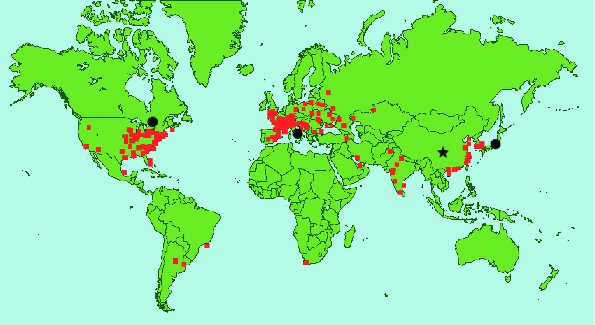
\includegraphics[width=1.0\textwidth]{figures/WorldMap.jpg}
    \caption{\label{fig:cjpl} Location of China JinPing Underground Laboratory}
\end{figure}
\end{minipage}
\begin{minipage}{.45\textwidth}
\begin{figure}[H]
    \centering
    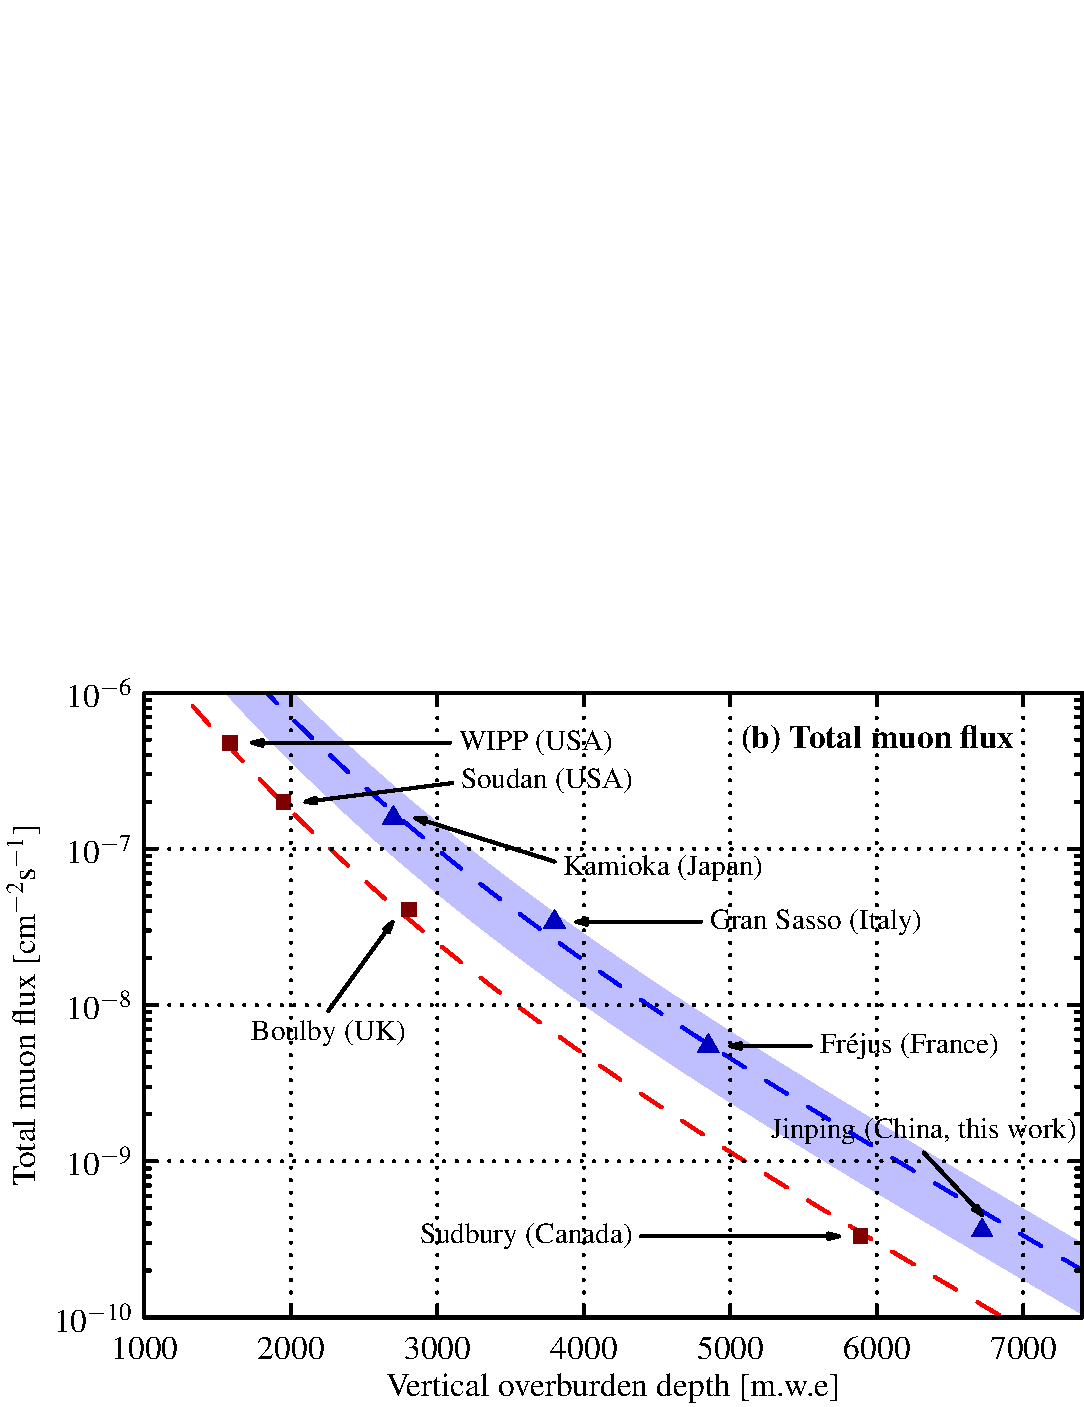
\includegraphics[width=1.0\textwidth]{figures/muonlab.pdf}
    \caption{\label{fig:muon} Total intensity of $\mu$ at different underground sites}
\end{figure}
\end{minipage}

There is an ongoing 1ton prototype (see figure~\ref{fig:1t}) in CJPL and next a hundred ton magnitude detector (see figure~\ref{fig:100t}) will be built and an 5000 tons detector (see figure~\ref{fig:1kt}) will be built in the future for Jinping Neutrino Experiment. 

\begin{minipage}{.3\textwidth}
\begin{figure}[H]
    \centering
    \includegraphics[width=0.8\linewidth]{figures/prototype.jpeg}
    \caption{\label{fig:1t} 1ton prototype}
\end{figure}
\end{minipage}
\begin{minipage}{.3\textwidth}
\begin{figure}[H]
    \centering
    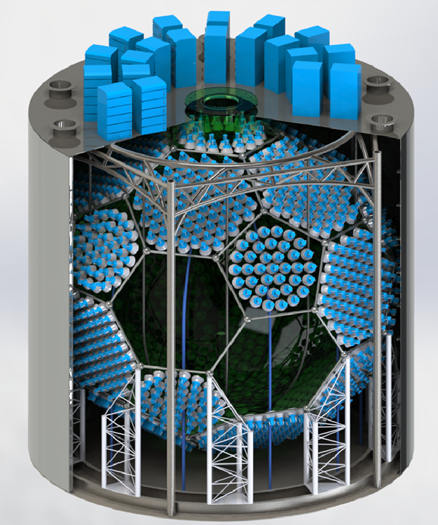
\includegraphics[width=0.8\linewidth]{figures/100tondetector.png}
    \caption{\label{fig:100t} $\sim$100t detector}
\end{figure}
\end{minipage}
\begin{minipage}{.3\textwidth}
\begin{figure}[H]
    \centering
    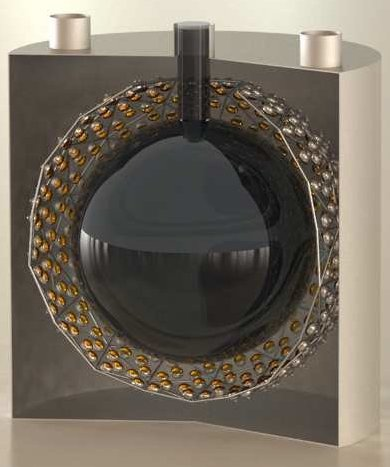
\includegraphics[width=0.8\linewidth]{figures/DetectoratJinping.jpg}
    \caption{\label{fig:1kt} $\sim$5000t detector}
\end{figure}
\end{minipage}

% section Jinping Neutrino Experiment (end)